\documentclass{article}

% Packages for formatting
\usepackage{tcolorbox}
\usepackage{xcolor}
\usepackage{hyperref}
\usepackage{amsmath}
\usepackage{geometry}
\usepackage{tocloft}
\usepackage{colortbl}
\usepackage{graphicx}
\usepackage{lipsum} % For dummy text
\usepackage{tikz}
\usepackage{listings}
\usepackage{tabularx}
\usepackage{float}
\usetikzlibrary{positioning}
\usetikzlibrary{shapes.geometric, arrows}

% Change hyperref settings to remove boxes
\hypersetup{
    colorlinks=true,
    linkcolor=black,
    filecolor=black,
    urlcolor=black,
    citecolor=black,
}

% Page layout
\geometry{a4paper, margin=1in}

% Colors
\definecolor{codehighlight}{rgb}{0.36, 0.54, 0.66}
\definecolor{coderule}{rgb}{0.7, 0.7, 0.7}           % Grey frame codebox
\definecolor{codebg}{rgb}{1.0, 1.0, 1.0}             % Background codebox
\definecolor{tableheader}{RGB}{128, 128, 128}        % Grey table header
\definecolor{tablecell}{RGB}{250, 250, 250}          % Table cell
\definecolor{title}{rgb}{0.36, 0.54, 0.66}           % Custom title color


% Code box style
\tcbset{
    colframe=tableheader, % Frame color
    colback=tablecell,    % Background color
    arc=0pt,           % Corner radius
    boxrule=1pt        % Frame thickness
}

% Table of contents
% \renewcommand{\cftbot}{}

% Main document
\begin{document}

% Cover pages
% Cover page
\begin{titlepage}
    \centering
    \vspace{\fill}  % push everything to top

    \thispagestyle{empty} % Remove page numbering

    % Background image
    \newgeometry{left=0cm, right=0cm, top=0cm, bottom=0cm} % Temporarily set margins to 0
    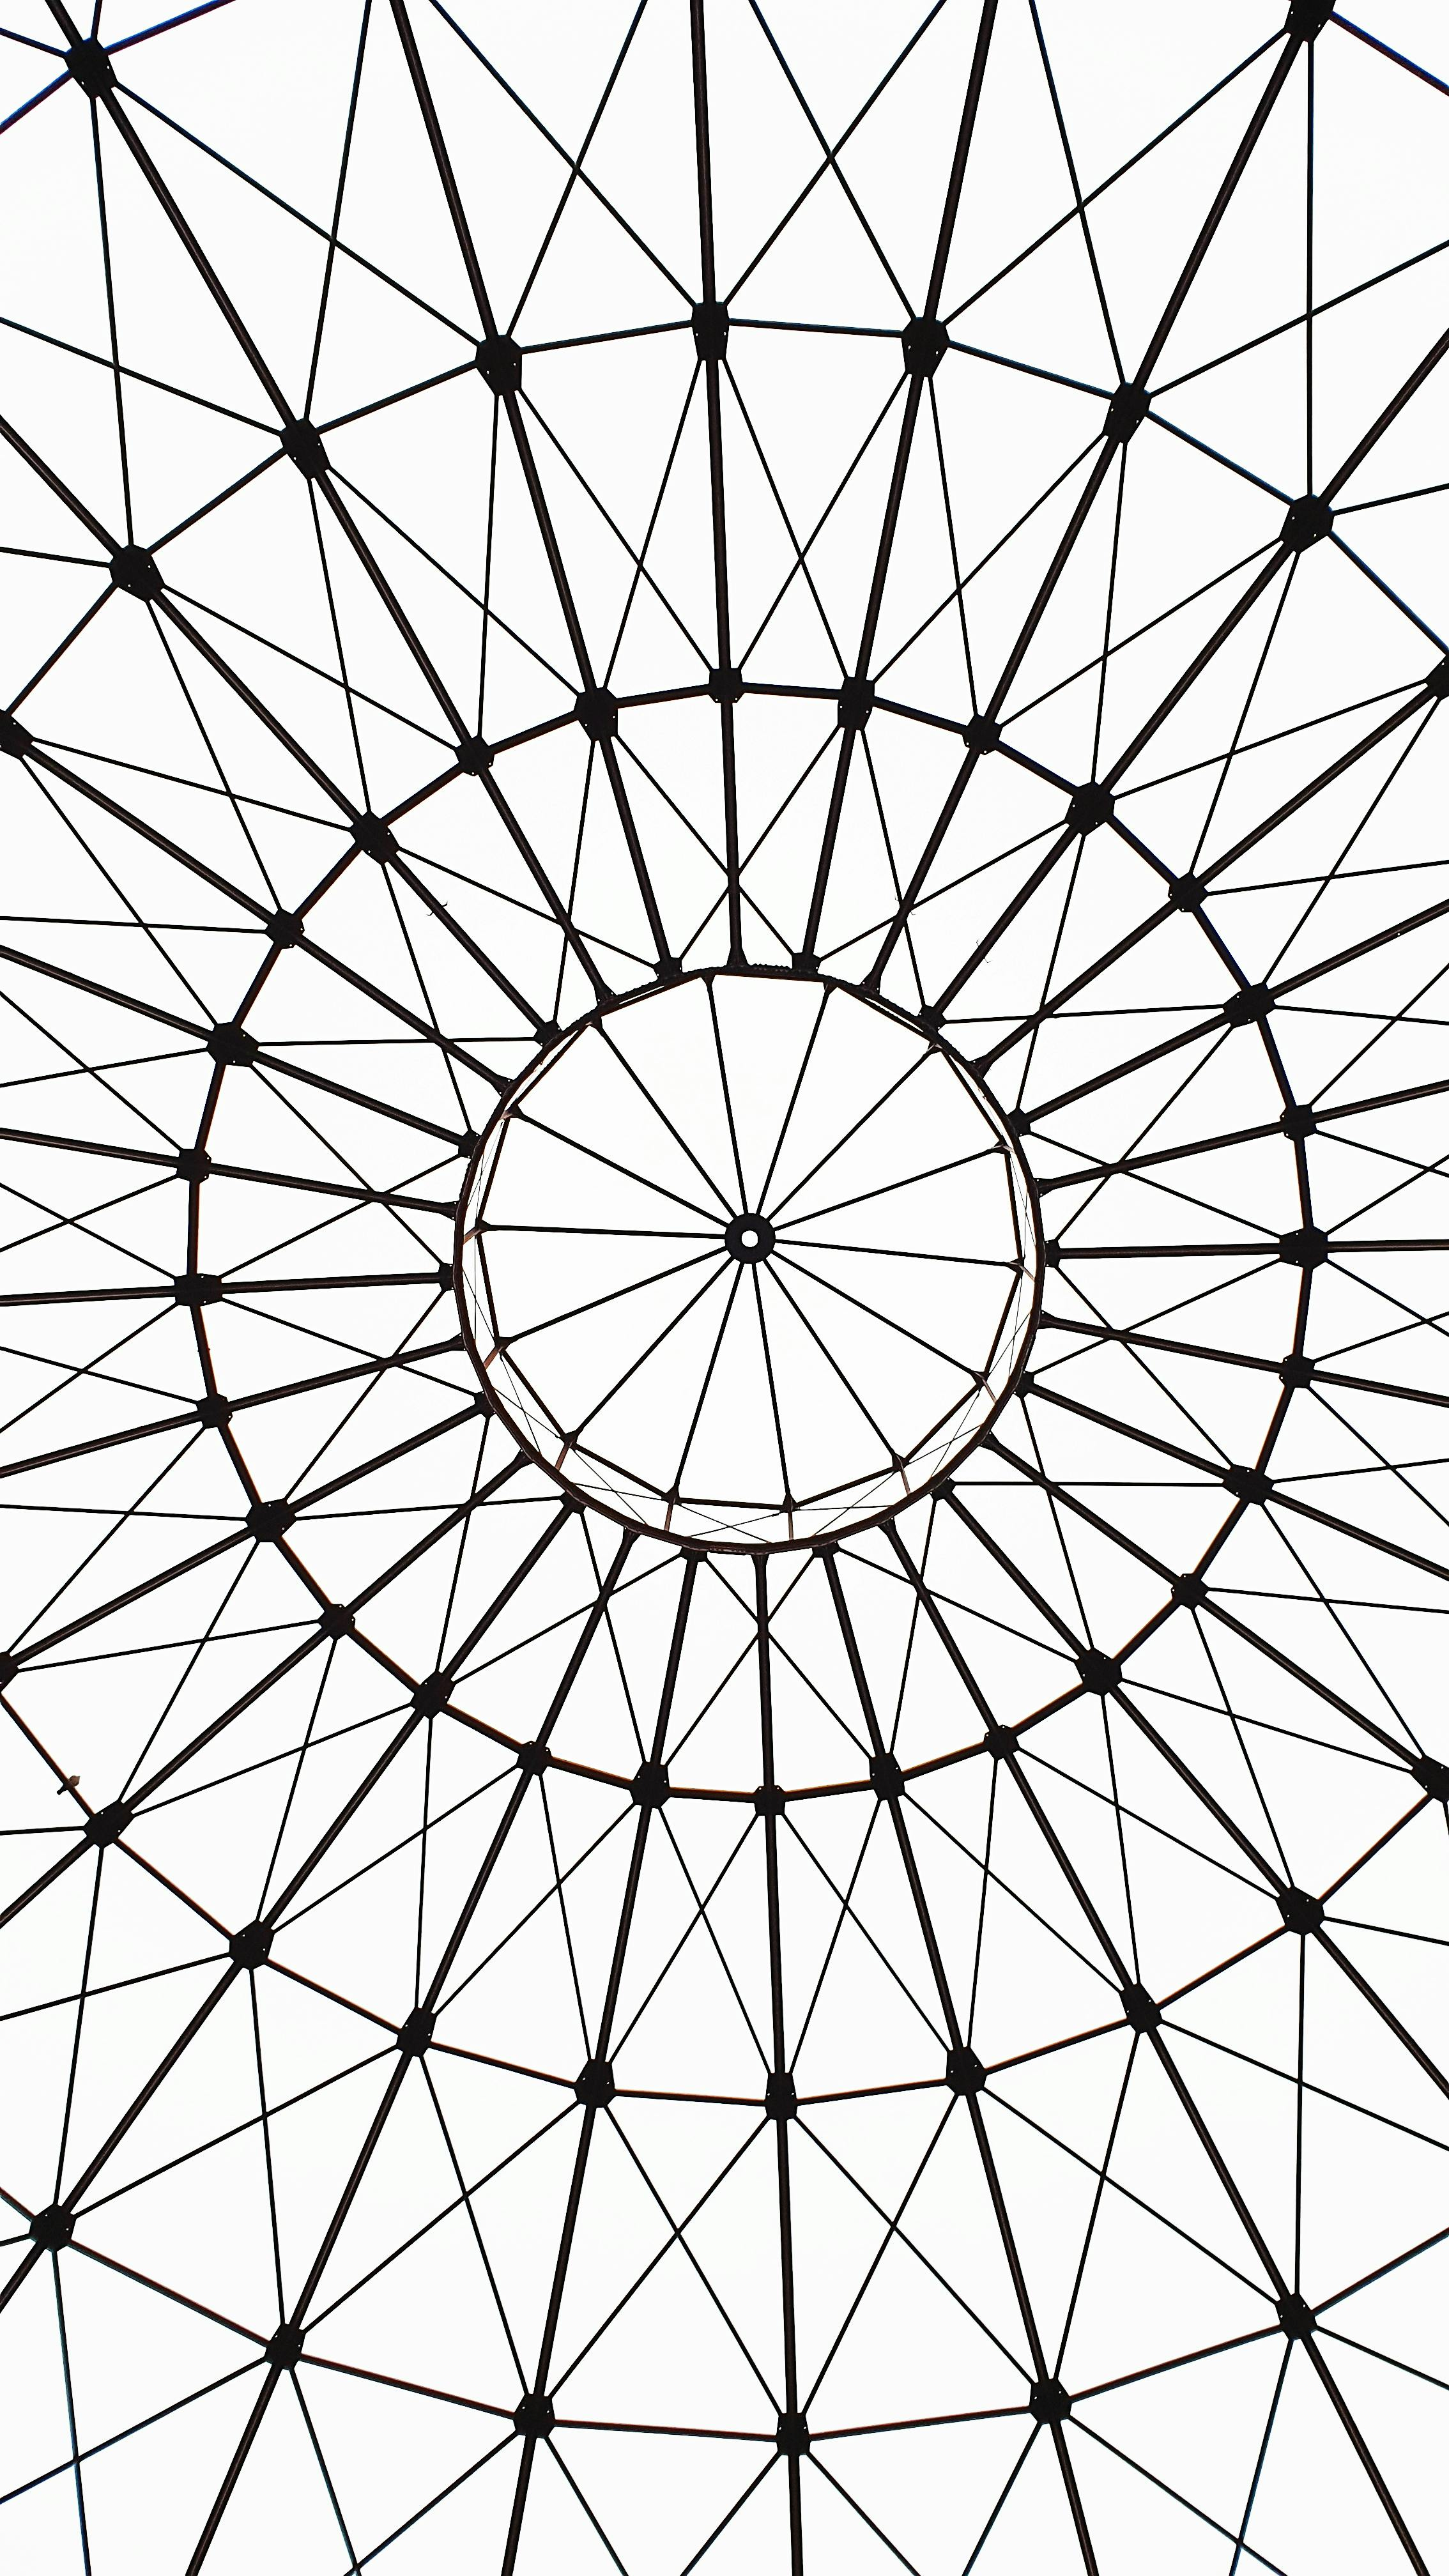
\includegraphics[width=\paperwidth,height=\paperheight]{images/cover.jpg}
    \restoregeometry % Restore the margins

    \vspace{\fill}   % push everything to bottom
\end{titlepage}
\newpage
\ % The empty page
\thispagestyle{empty} % Remove page numbering
\newpage
% Title page
\begin{titlepage}
    \thispagestyle{empty} % Remove page numbering
    \centering
    \vfill                % push everything to top
    \begin{center}
        {\Huge \textbf{C++ QuestionBank}}\\
        \vspace{1cm}
        {\Large Anchit Mulye}\\
        \vspace{0.5cm}
        {\Large \today}
    \end{center}
    \vfill                % push everything to bottom
\end{titlepage}
\newpage
\ % The empty page
\thispagestyle{empty} % Remove page numbering
\newpage
\pagenumbering{roman}
% Table of contents
\newpage
\thispagestyle{empty} % Remove page numbering
\title{C++ Question Bank}
\author{Anchit Mulye}
\date{\today}
\maketitle

\tableofcontents
\newpage

% Chapters
\pagenumbering{arabic}
\section{Basic of C++}

\subsection{What are the key features of C++?}
\begin{itemize}
    \item \textbf{Object-Oriented:} Supports object-oriented programming paradigms like classes, inheritance, polymorphism, and encapsulation.
    \item \textbf{Rich Standard Library:} Provides a comprehensive library that includes algorithms, containers, and functions for various tasks.
    \item \textbf{Performance:} Offers low-level control over hardware and memory, making it suitable for system-level programming and performance-critical applications.
    \item \textbf{Portability:} Designed to be platform-independent, with compilers available for most operating systems.
    \item \textbf{Compatibility:} Supports both procedural and object-oriented programming, enabling developers to choose the appropriate paradigm based on project requirements.
    \item \textbf{Memory Management:} Supports both static and dynamic memory allocations.
\end{itemize}

\subsection{Explain the structure of a C++ program.}
A typical C++ program consists of the following components:
\begin{itemize}
    \item \textbf{Preprocessor Directives:} These are instructions to the preprocessor, which processes the source code before compilation. Directives start with \texttt{\#} and include commands like \texttt{\#include} for including header files.
    \item \textbf{Namespace Declaration:} Namespaces help avoid name collisions and organize code. The \texttt{namespace} keyword declares a scope where identifiers can exist.
    \item \textbf{Main Function:} Every C++ program must have a \texttt{main()} function, which serves as the entry point. Execution of the program begins from \texttt{main()}.
    \item \textbf{Variable Declarations:} Variables are declared to store data. They must be declared before they are used, specifying the data type.
    \item \textbf{Statements and Expressions:} C++ statements perform actions, and expressions compute values. These form the core logic of the program.
    \item \textbf{Functions:} Functions encapsulate reusable code. They are declared with a return type, name, parameters (optional), and a function body.
    \item \textbf{Classes and Objects (Optional):} C++ supports object-oriented programming. Classes define data structures and methods, while objects are instances of classes.
    \item \textbf{Comments:} Comments improve code readability and understanding. They can be single-line (\texttt{//}) or multi-line (\texttt{/* */}).
    \item \textbf{Headers and Libraries:} Header files (\texttt{\#include}) provide declarations needed for compilation. Libraries extend functionality beyond standard C++.
    \item \textbf{End of Program:} The \texttt{return} statement in \texttt{main()} (if required) signifies the end of the program execution, returning an exit status to the operating system.
\end{itemize}

\subsection{Explain the steps from source code to executable.}
\begin{itemize}
    \item \textbf{Source Code (\texttt{.cpp} files):} This is where you write your C++ program using a text editor or an Integrated Development Environment (IDE).
    \item \textbf{Preprocessing:}
    \begin{itemize}
        \item \textbf{Tool:} Preprocessor
        \item \textbf{Description:} Before compilation begins, the preprocessor handles directives starting with \texttt{\#}, such as \texttt{\#include} and \texttt{\#define}. It includes header files and expands macros to generate an intermediary file (\texttt{.i}).
    \end{itemize}
    \item \textbf{Compilation:}
    \begin{itemize}
        \item \textbf{Tool: Compiler (\texttt{g++}, \texttt{clang++}, etc.)}
        \item \textbf{Description:} The compiler translates the preprocessed source code (\texttt{.i} file) into assembly language code (\texttt{.s} file). It checks syntax, semantics, and type correctness during this phase.
    \end{itemize}
    \item \textbf{Assembly:}
    \begin{itemize}
        \item \textbf{Tool: Assembler (as)}
        \item \textbf{Description:} The assembler converts the assembly code (\texttt{.s} file) into machine code or object code (\texttt{.o} file). Each line of assembly code corresponds directly to a machine instruction.
    \end{itemize}
    \item \textbf{Linking:}
    \begin{itemize}
        \item \textbf{Tool: Linker (ld)}
        \item \textbf{Description:} The linker combines multiple object files (\texttt{.o} files) generated from the compilation step along with necessary libraries (like the C++ Standard Library) to create a single executable file. It resolves external references between files, assigns addresses to variables and functions, and generates the final executable (\texttt{.exe} on Windows, without extension on Unix-like systems).
    \end{itemize}
    \item \textbf{Loading (Optional):}
    \begin{itemize}
        \item \textbf{Tool:} Loader
        \item \textbf{Description:} On some operating systems, an additional loading step may occur where the executable is loaded into memory for execution.
    \end{itemize}
    \item \textbf{Execution:}
    \begin{itemize}
        \item \textbf{Tool:} Operating System
        \item \textbf{Description:} Finally, the operating system loads the executable into memory and starts executing the \texttt{main()} function, initiating the program.
    \end{itemize}
\end{itemize}
\begin{tcolorbox}[arc=5pt, boxrule=2pt, title=Notes]
    \begin{itemize}
    \item \textbf{Header Files:} These are included in the preprocessing step (\texttt{\#include}) and provide declarations for functions, classes, and constants used in the program.
    \item \textbf{Libraries:} Besides standard libraries, you can link external libraries (static \texttt{.lib} or dynamic \texttt{.dll/.so}) to extend functionality.
    \item \textbf{Debugging Symbols:} Debug versions of executables may include symbols (\texttt{pdb} on Windows, \texttt{dSYM} on macOS) to aid in debugging.
    \end{itemize}
\end{tcolorbox}

\subsection{What are data types in C++?}
\begin{itemize}
    \item \textbf{Primitive Data Types:} Integer, Float, Character, Boolean, Void
    \item \textbf{Derived Data Types:} Pointers, References, Functions, Arrays
    \item \textbf{User Defined Data Types:} Classes, Structures, Unions, Enumerations
\end{itemize}

\subsection{What is call by value and call by reference?}
\begin{itemize}
    \item \textbf{Call by Value:} a copy of the actual argument is passed to the function.
    \begin{tcolorbox}[title=Call by Value]
    \begin{verbatim}
    void modifyValue(int value) {
        value = 100; // Change local copy
    }
    
    int main() {
        int a = 10;
        modifyValue(a); // Pass by value
        std::cout << "Value after: " << a << std::endl; // a remains 10
        return 0;
    }
    \end{verbatim}
    \end{tcolorbox}
    \item \textbf{Call by Reference:} a reference to the actual argument is passed to the function.
    \begin{tcolorbox}[title=Call by Reference]
    \begin{verbatim}
    void modifyValue(int &value) {
        value = 100; // Change original value
    }

    int main() {
        int a = 10;
        modifyValue(a); // Pass by reference
        std::cout << "Value after: " << a << std::endl; // a becomes 100
        return 0;
    }
    \end{verbatim}
    \end{tcolorbox}
    \item \textbf{Call by Pointer:} similar to call by reference, but with pointers.
    \begin{tcolorbox}[title=Call by Pointer]
    \begin{verbatim}
    void modifyValue(int *value) {
        *value = 100; // Change original value via pointer
    }

    int main() {
        int a = 10;
        modifyValue(&a); // Pass by pointer
        std::cout << "Value after: " << a << std::endl; // a becomes 100
        return 0;
    }
    \end{verbatim}
    \end{tcolorbox}
\end{itemize}


\subsection{What are differences between pass by value and pass by reference?}
\begin{table}[H]
    \centering
    \begin{tabularx}{\textwidth}{|p{2.5cm}|X|X|}
    \hline \rowcolor{tableheader}
    \textbf{}                    & \textbf{Pass by Value}            & \textbf{Pass by Reference} \\
    \hline \textbf{Memory}       & Higher memory usage due to copies & Lower memory usage, only references are passed \\
    \hline \textbf{Performance}  & Potentially slower due to copying & Generally faster, no copying involved \\
    \hline \textbf{Effects}      & No effect on original data        & Modifies the original data \\
    \hline \textbf{Safety}       & Safer, no unintended side effects & Riskier, careful handling required to avoid issues \\
    \hline
    \end{tabularx}
\end{table}

\subsection{What are differences between reference and pointer?}
\begin{table}[H]
    \centering
    \begin{tabularx}{\textwidth}{|p{2.5cm}|X|X|}
    \hline \rowcolor{tableheader}
    \textbf{}                      & \textbf{Reference}                      & \textbf{Pointer} \\
    \hline \textbf{Syntax}         & \texttt{int \&ref = variable}           & \texttt{int *ptr = \&variable} \\
    \hline \textbf{Initialization} & Must be initialized and can not be null & Can be declared without initialization and can be null \\
    \hline \textbf{Reassignment}   & Reference cannot be changed             & Can be reassigned to point to a different variable \\
    \hline \textbf{Dereferencing}  & Automatically dereferenced              & Explicit dereferencing using \texttt{*int value = *ptr} \\
    \hline \textbf{Address}        & Does not have its own address           & Has its own address and can store other addresses \\
    \hline \textbf{Use Cases}      & Function parameters and return values; Operator overloading   & Dynamic memory allocation; Low level memory manipulation \\
    \hline 
    \end{tabularx}
\end{table}

\subsection{What are differences between prefix and postfix?}
\begin{itemize}
    \item \textbf{Prefix Increment/Decrement}
        \begin{itemize}
        \item \textbf{Syntax:} \texttt{++variable} or \texttt{--variable}
        \item \textbf{Operation:} The operator is applied before the value is used in the expression.
        \end{itemize}
    \begin{tcolorbox}[title=Prefix]
    \begin{verbatim}
    int a = 5;
    int b = ++a; // a is incremented to 6, then b is assigned the value 6
    \end{verbatim}
    \end{tcolorbox}
    \item \textbf{Postfix Increment/Decrement}
        \begin{itemize}
        \item \textbf{Syntax:} \texttt{variable++} or \texttt{variable--}
        \item \textbf{Operation:} The operator is applied after the value is used in the expression.
        \end{itemize} 
    \begin{tcolorbox}[title=Postfix]
    \begin{verbatim} 
    int a = 5;
    int b = a++; // b is assigned the value 5, then a is incremented to 6
    \end{verbatim}
    \end{tcolorbox}
\end{itemize}

\subsection{What are operations on pointers?}
\begin{itemize}
    \item Declaration and Initialization
    \item Assignment
    \item Dereferencing
    \item Address-of Operator
    \item Pointer Arithmetic
    \item Comparison
    \item Null Pointers
\end{itemize}
\begin{tcolorbox}[title=Operations on Pointers]
    \begin{verbatim}
    #include <iostream>

    int main() {
        int x = 10;
        int y = 20;
        int arr[] = {1, 2, 3, 4, 5};
    
        // Declaration and Initialization
        int *ptr1 = &x;
        int *ptr2 = &y;
    
        // Assignment
        ptr1 = ptr2; // ptr1 now points to y
    
        // Dereferencing
        std::cout << "Value at ptr1: " << *ptr1 << std::endl; // Output: 20
        *ptr1 = 30; // Changing the value of y to 30
    
        // Address-of Operator
        int *ptr3 = &x;
    
        // Pointer Arithmetic
        int *ptrArr = arr;
        std::cout << "First element: " << *ptrArr << std::endl; // Output: 1
        ptrArr++;
        std::cout << "Second element: " << *ptrArr << std::endl; // Output: 2
    
        // Comparison
        if (ptr1 != ptr2) {
            std::cout << "Pointers are different" << std::endl;
        } else {
            std::cout << "Pointers are the same" << std::endl; // Printed
        }
    
        // Null Pointer
        int *ptrNull = nullptr;
        if (ptrNull == nullptr) {
            std::cout << "ptrNull is a null pointer" << std::endl; // Printed
        }
    
        return 0;
    }        
    \end{verbatim}
\end{tcolorbox}

\subsection{What are different storage classes?}
In C++, storage classes define the scope, visibility, and lifetime of variables and/or functions within a C++ program. There are four storage classes in C++:

\begin{itemize}
    \item \textbf{\texttt{auto}}:
    \begin{itemize}
        \item Default storage class for local variables.
        \item The variable is only visible within the block where it is defined.
    \end{itemize}
    \item \textbf{\texttt{register}}:
    \begin{itemize}
        \item Suggests that the variable be stored in a CPU register instead of RAM.
        \item Used for variables that require fast access.
    \end{itemize}
    \item \textbf{\texttt{static}}:
    \begin{itemize}
        \item The variable retains its value between multiple function calls.
        \item For global variables, the variable is limited to the file scope.
    \end{itemize}
    \item \textbf{\texttt{extern}}:
    \begin{itemize}
        \item Used to declare a global variable or function in another file.
        \item Indicates that the variable is defined elsewhere.
    \end{itemize}
    \item \textbf{\texttt{mutable}}:
    \begin{itemize}
        \item Allows a member of an object to be modified even if the object is const.
        \item Used primarily with class member variables.
    \end{itemize}
\end{itemize}

\subsection{What are access modifiers?}
Access modifiers in C++ are keywords that set the access level or visibility of class members. There are three primary access modifiers:

\begin{itemize}
    \item \textbf{\texttt{public}}:
    \begin{itemize}
        \item Members are accessible from outside the class.
        \item Used for functions and variables that need to be accessed by other classes.
    \end{itemize}
    \item \textbf{\texttt{protected}}:
    \begin{itemize}
        \item Members are accessible within the class and by derived class instances.
        \item Used to allow derived classes to access the base class members while hiding them from the rest of the program.
    \end{itemize}
    \item \textbf{\texttt{private}}:
    \begin{itemize}
        \item Members are only accessible within the class itself.
        \item Used to hide data and functions from outside the class.
    \end{itemize}
\end{itemize}

\subsection{What are inline functions}
Inline functions are functions defined with the \texttt{inline} keyword, which suggests to the compiler to insert the function's code at the point of call rather than performing a traditional function call. This can improve performance by avoiding the overhead of a function call, especially for small, frequently called functions.

\begin{itemize}
    \item Declared using the \texttt{inline} keyword.
    \item Useful for small functions that are called frequently.
    \item Can lead to faster execution but may increase the size of the binary.
    \begin{tcolorbox}[title=Inline Function]
    \begin{verbatim}
    inline int add(int a, int b) {
        return a + b;
    }
    \end{verbatim}
    \end{tcolorbox}
\end{itemize}

\subsection{What are differences between \texttt{static} and \texttt{volatile}?}
\begin{itemize}
    \item \textbf{\texttt{static}}:
    \begin{itemize}
        \item The \texttt{static} keyword in C++ is used to declare variables that retain their value between function calls.
        \item It can be applied to local variables, global variables, and class members.
        \item A \texttt{static} variable inside a function retains its value between invocations of the function.
        \item A \texttt{static} global variable or function has internal linkage, meaning it is only accessible within the file in which it is declared.
        \item A \texttt{static} class member is shared among all instances of the class.
    \end{itemize}
    
    \item \textbf{\texttt{volatile}}:
    \begin{itemize}
        \item The \texttt{volatile} keyword is used to indicate that a variable's value may be changed at any time by something outside the control of the code section in which it appears.
        \item This prevents the compiler from optimizing the code in ways that assume the variable's value is not changing unexpectedly.
        \item It is commonly used in embedded systems, multithreading, and signal handling.
    \end{itemize}
\end{itemize}

\subsection{Explain the concept of RAII (Resource Acquisition Is Initialization).}
Resource Acquisition Is Initialization (RAII) is a programming idiom used to manage resources such as memory, file handles, and network connections. It ties resource management to the lifetime of objects, ensuring that resources are properly released when objects go out of scope.

\begin{itemize}
    \item Resources are acquired and released by constructors and destructors, respectively.
    \item Ensures exception safety by automatically releasing resources in the destructor.
    \item Commonly used with smart pointers, file streams, and lock guards.
\end{itemize}

\subsection{What is exception handling in C++? Why is it used?}
Exception handling in C++ provides a way to react to exceptional circumstances (errors) in a program. It is used to manage errors and exceptional conditions in a controlled way, allowing the program to continue running or gracefully terminate.

\begin{itemize}
    \item Helps in separating error-handling code from regular code.
    \item Enables handling of runtime errors, preventing abrupt program termination.
\end{itemize}

\subsection{Explain the \texttt{try}, \texttt{catch}, and \texttt{throw} blocks in C++.}
\begin{itemize}
    \item \textbf{\texttt{try}} block:
    \begin{itemize}
        \item Contains code that might throw an exception.
        \item If an exception is thrown, the control is transferred to the corresponding \texttt{catch} block.
    \end{itemize}
    
    \item \textbf{\texttt{catch}} block:
    \begin{itemize}
        \item Used to handle exceptions thrown by the \texttt{try} block.
        \item Multiple \texttt{catch} blocks can be used to handle different types of exceptions.
    \end{itemize}
    
    \item \textbf{\texttt{throw}} statement:
    \begin{itemize}
        \item Used to throw an exception.
        \item Can be used to throw exceptions of any type.
    \end{itemize}
\end{itemize}
\begin{tcolorbox}[title=Exception Handling]
\begin{verbatim}
    try {
        // Code that may throw an exception
        throw std::runtime_error("Error occurred");
    } catch (const std::runtime_error &e) {
        // Handle runtime error
        std::cerr << e.what() << std::endl;
    } catch (...) {
        // Handle any exception
        std::cerr << "Unknown error" << std::endl;
    }
\end{verbatim}        
\end{tcolorbox}

\subsection{What is the difference between runtime error and compile time error?}
\begin{itemize}
    \item \textbf{Runtime Error}:
    \begin{itemize}
        \item Occurs during the execution of a program.
        \item Examples include division by zero, null pointer dereference, and out-of-bounds array access.
        \item Usually leads to program termination or undefined behavior.
    \end{itemize}

    \item \textbf{Compile Time Error}:
    \begin{itemize}
        \item Detected by the compiler during the compilation of the program.
        \item Examples include syntax errors, type mismatches, and undeclared variables.
        \item Prevents the program from compiling successfully.
    \end{itemize}
\end{itemize}

\subsection{How do you create a custom exception in C++?}
Creating a custom exception in C++ involves defining a new class that inherits from the \texttt{std::exception} class or any of its derived classes.
\begin{tcolorbox}[title=Custom Exception]
\begin{verbatim}
#include <exception>

class MyCustomException : public std::exception {
public:
    const char* what() const noexcept override {
        return "My custom exception occurred";
    }
};

int main() {
    try {
        throw MyCustomException();
    } catch (const MyCustomException &e) {
        std::cerr << e.what() << std::endl;
    }
    return 0;
}
\end{verbatim}
\end{tcolorbox}

\subsection{How do you open and close a file in C++?}
To open and close a file in C++, you use the file stream classes from the \texttt{<fstream>} library.
\begin{tcolorbox}[title=File Open and Close]
\begin{verbatim}
#include <fstream>
#include <iostream>

int main() {
    std::ofstream outFile("example.txt"); // Open file for writing
    if (outFile.is_open()) {
        outFile << "Writing to file\n";
        outFile.close(); // Close the file
    }

    std::ifstream inFile("example.txt"); // Open file for reading
    if (inFile.is_open()) {
        std::string line;
        while (std::getline(inFile, line)) {
            std::cout << line << std::endl;
        }
        inFile.close(); // Close the file
    }

    return 0;
}
\end{verbatim}
\end{tcolorbox}

\subsection{Explain the difference between \texttt{ifstream}, \texttt{ofstream}, and \texttt{fstream} in C++.}
\begin{itemize}
    \item \textbf{\texttt{ifstream}}:
    \begin{itemize}
        \item Input file stream.
        \item Used for reading from files.
    \end{itemize}
    
    \item \textbf{\texttt{ofstream}}:
    \begin{itemize}
        \item Output file stream.
        \item Used for writing to files.
    \end{itemize}
    
    \item \textbf{\texttt{fstream}}:
    \begin{itemize}
        \item File stream.
        \item Used for both reading from and writing to files.
    \end{itemize}
\end{itemize}

\subsection{How do you check if a file exists in C++?}
To check if a file exists in C++, you can use the \texttt{std::ifstream} class.

\begin{tcolorbox}[title=File Exists]
\begin{verbatim}
#include <fstream>
#include <iostream>

bool fileExists(const std::string &filename) {
    std::ifstream file(filename);
    return file.good();
}

int main() {
    std::string filename = "example.txt";
    if (fileExists(filename)) {
        std::cout << "File exists.\n";
    } else {
        std::cout << "File does not exist.\n";
    }
    return 0;
}
\end{verbatim}
\end{tcolorbox}

\subsection{What is the difference between \texttt{const char*}, \texttt{char* const}, and \texttt{const char* const}.}
\begin{itemize}
    \item \textbf{\texttt{const char*}}:
    \begin{itemize}
        \item Pointer to a constant character.
        \item The character pointed to by the pointer cannot be modified.
        \item The pointer itself can be modified to point to another character.
        \item Example: \texttt{const char* ptr = "Hello";}
    \end{itemize}
    
    \item \textbf{\texttt{char* const}}:
    \begin{itemize}
        \item Constant pointer to a character.
        \item The pointer itself cannot be modified after initialization.
        \item The character pointed to by the pointer can be modified.
        \item Example: \texttt{char c = 'A'; char* const ptr = \&c;}
    \end{itemize}
    
    \item \textbf{\texttt{const char* const}}:
    \begin{itemize}
        \item Constant pointer to a constant character.
        \item Neither the pointer nor the character it points to can be modified.
        \item Example: \texttt{const char* const ptr = "Hello";}
    \end{itemize}
\end{itemize}

\subsection{How to return a string from a function in C++?}
\begin{itemize}
\item \textbf{Method 1: Returning a String Object}
\begin{tcolorbox}[title=As an Object]
\begin{verbatim}
#include <iostream>
#include <string>

std::string getString() {
    std::string message = "Hello, World!";
    return message;
}

int main() {
    std::string result = getString();
    std::cout << "Returned string: " << result << std::endl;
    return 0;
}
\end{verbatim}
\end{tcolorbox}

\item \textbf{Method 2: Returning a String by Reference}
\begin{tcolorbox}[title=As a Reference]
\begin{verbatim}
#include <iostream>
#include <string>

const std::string& getString() {
    static std::string message = "Hello, World!";
    return message;
}

int main() {
    const std::string& result = getString();
    std::cout << "Returned string: " << result << std::endl;
    return 0;
}
\end{verbatim}
\end{tcolorbox}
\end{itemize}

\subsection{What are namespaces in C++? Explain how they work.}

Namespaces are a feature in C++ that allows you to group a set of related classes, functions, and variables under a single name. This helps to avoid name collisions in large projects where multiple libraries might have functions or variables with the same names. By encapsulating these entities within a namespace, you ensure that their names are unique within the scope of that namespace.
Here is a basic example to illustrate how namespaces work in C++:
\begin{tcolorbox}[title=Namespace]
\begin{verbatim}
#include <iostream>

namespace MyNamespace {
    void display() {
        std::cout << "Hello from MyNamespace!" << std::endl;
    }
}

int main() {
    MyNamespace::display();
    return 0;
}
\end{verbatim}
\end{tcolorbox}

\begin{itemize}
    \item \textbf{Declaration:} The keyword \texttt{namespace} is used to declare a namespace. In this example, \texttt{MyNamespace} is a namespace that contains the \texttt{display} function.
    \item \textbf{Scope Resolution Operator:} To call a function or access a variable within a namespace, you use the scope resolution operator \texttt{::}. In \texttt{MyNamespace::display()}, the \texttt{::} operator is used to access the \texttt{display} function within \texttt{MyNamespace}.
\end{itemize}

\textbf{Types of Namespaces}
\begin{itemize}
    \item Regular Namespaces
    \item Anonymous Namespaces
    \item Nested Namespaces
    \item Inline Namespaces (C++11 and later)
    \item Standard Namespace
\end{itemize}

\subsection{}
\subsection{}
\subsection{}
\subsection{}
\section{Arrays}

\subsection{Write a program to find the intersection of two arrays.}
\begin{tcolorbox}[title=]
\begin{verbatim}
std::vector<int> findIntersection(const std::vector<int>& arr1, 
                                    const std::vector<int>& arr2) {
    std::unordered_set<int> set(arr1.begin(), arr1.end());
    std::vector<int> intersection;

    for (int num : arr2) {
        if (set.count(num)) {
            intersection.push_back(num);
            set.erase(num); // to handle duplicates in arr2
        }
    }

    return intersection;
}
\end{verbatim}
\end{tcolorbox}

\subsection{Write a program to find the union of two arrays.}
\begin{tcolorbox}[title=]
\begin{verbatim}
std::vector<int> findUnion(const std::vector<int>& arr1, 
                            const std::vector<int>& arr2) {
    std::unordered_set<int> set(arr1.begin(), arr1.end());

    for (int num : arr2) {
        set.insert(num);
    }

    std::vector<int> union_vec(set.begin(), set.end());
    return union_vec;
}    
\end{verbatim}
\end{tcolorbox}

\subsection{Write a program to remove duplicates from an array.}
\begin{tcolorbox}[title=]
\begin{verbatim}
std::vector<int> removeDuplicates(const std::vector<int>& arr) {
    std::unordered_set<int> set;
    std::vector<int> unique;

    for (int num : arr) {
        if (set.insert(num).second) { // insert means num was not in the set
            unique.push_back(num);
        }
    }

    return unique;
}
\end{verbatim}
\end{tcolorbox}

\subsection{Write a program to find the second largest number in an array.}
\begin{tcolorbox}[title=]
\begin{verbatim}
int findSecondLargest(const std::vector<int>& arr) {
    int first = INT_MIN;
    int second = INT_MIN;

    for (int num : arr) {
        if (num > first) {
            second = first;
            first = num;
        } else if (num > second && num != first) {
            second = num;
        }
    }

    return second;
}
\end{verbatim}
\end{tcolorbox}

\subsection{Write a program to find the median of an array of numbers.}
\begin{tcolorbox}[title=]
\begin{verbatim}
double findMedian(std::vector<int>& arr) {
    size_t n = arr.size();
    std::sort(arr.begin(), arr.end());

    if (n % 2 == 0) {
        return (static_cast<double>(arr[n/2 - 1]) +
                 static_cast<double>(arr[n/2])) / 2.0;
    } else {
        return static_cast<double>(arr[n/2]);
    }
}    
\end{verbatim}
\end{tcolorbox}

\subsection{Write a program to find the maximum and minimum elements in an array.}
\begin{tcolorbox}[title=]
\begin{verbatim}
void findMinMax(const std::vector<int>& arr, int& min, int& max) {
    min = INT_MAX;
    max = INT_MIN;

    for (int num : arr) {
        if (num < min) min = num;
        if (num > max) max = num;
    }
}
\end{verbatim}
\end{tcolorbox}

\section{Strings}

\subsection{Write a program to check if a string is a palindrome.}
\begin{tcolorbox}[title=]
\begin{verbatim}
bool isPalindrome(string s) {
    int left = 0, right = s.length() - 1;
    while (left < right) {
        if (s[left] != s[right])
            return false;
        left++;
        right--;
    }
    return true;
}
\end{verbatim}
\end{tcolorbox}

\subsection{Write a program to find the ASCII value of a character.}
\begin{tcolorbox}[title=]
\begin{verbatim}
int getAsciiValue(char c) {
    return int(c);
}
\end{verbatim}
\end{tcolorbox}

\subsection{Write a program to convert string to number.}
\begin{tcolorbox}[title=]
\begin{verbatim}
int stringToNumber(const std::string& str) {
    std::stringstream ss(str);
    int num;
    ss >> num;
    return num;
}
\end{verbatim}
\end{tcolorbox}

\subsection{Write a program to check if a string contains only digits.}
\begin{tcolorbox}[title=]
\begin{verbatim}
bool containsOnlyDigits(const std::string& str) {
    for (char c : str) {
        if (!isdigit(c)) {
            return false;
        }
    }
    return true;
}
\end{verbatim}
\end{tcolorbox}

\subsection{Write a program to check if two strings are anagrams of each other.}
\begin{tcolorbox}[title=]
\begin{verbatim}
bool areAnagrams(const std::string& str1, const std::string& str2) {
    std::string s1 = str1;
    std::string s2 = str2;
    std::sort(s1.begin(), s1.end());
    std::sort(s2.begin(), s2.end());
    return (s1 == s2);
}
\end{verbatim}
\end{tcolorbox}

\subsection{Write a program to reverse a string.}
\begin{tcolorbox}[title=]
\begin{verbatim}
std::string reverseString(const std::string& str) {
    std::string reversed = str;
    std::reverse(reversed.begin(), reversed.end());
    return reversed;
}
\end{verbatim}
\end{tcolorbox}

\subsection{Write a program to check if a string is a pangram (contains every letter of the alphabet at least once).}
\begin{tcolorbox}[title=]
\begin{verbatim}
bool isPangram(const std::string& str) {
    bool letters[26] = {false};
    int index;

    for (char c : str) {
        if (isalpha(c)) {
            if (islower(c)) {
                index = c - 'a';
            } else {
                index = c - 'A';
            }
            letters[index] = true;
        }
    }

    for (int i = 0; i < 26; ++i) {
        if (!letters[i]) {
            return false;
        }
    }

    return true;
}
\end{verbatim}
\end{tcolorbox}

\subsection{Write a program to check if a string is an anagram of a palindrome.}
\begin{tcolorbox}[title=]
\begin{verbatim}
bool canFormPalindrome(const std::string& str) {
    std::unordered_map<char, int> freq;
    int oddCount = 0;

    for (char c : str) {
        freq[c]++;
    }

    for (auto& pair : freq) {
        if (pair.second % 2 != 0) {
            oddCount++;
        }
    }

    return (oddCount <= 1);
}
\end{verbatim}
\end{tcolorbox}
\section{Data Structures}

\subsection{Write a program to implement a stack (using arrays or linked lists).}
\begin{tcolorbox}[title=]
\begin{verbatim}
#define MAX_SIZE 100

class Stack {
private:
    int arr[MAX_SIZE];
    int top;

public:
    Stack() {
        top = -1;
    }

    void push(int value) {
        if (top >= MAX_SIZE - 1) {
            cout << "Stack Overflow\n";
            return;
        }
        arr[++top] = value;
    }

    int pop() {
        if (top < 0) {
            cout << "Stack Underflow\n";
            return -1; // or throw an exception
        }
        return arr[top--];
    }

    int peek() {
        if (top < 0) {
            cout << "Stack is empty\n";
            return -1; // or throw an exception
        }
        return arr[top];
    }

    bool isEmpty() {
        return (top == -1);
    }
};

int main() {
    Stack s;
    s.push(10);
    s.push(20);
    s.push(30);
    cout << s.pop() << " popped from stack\n";
    cout << "Top element is " << s.peek() << endl;
}    
\end{verbatim}
\end{tcolorbox}

\subsection{Write a program to implement a queue (using arrays or linked lists).}
\begin{tcolorbox}[title=]
\begin{verbatim}
#define MAX_SIZE 100

class Queue {
private:
    int arr[MAX_SIZE];
    int front, rear;

public:
    Queue() {
        front = -1;
        rear = -1;
    }

    void enqueue(int value) {
        if (rear >= MAX_SIZE - 1) {
            cout << "Queue Overflow\n";
            return;
        }
        arr[++rear] = value;
        if (front == -1) {
            front = 0;
        }
    }

    int dequeue() {
        if (front == -1 || front > rear) {
            cout << "Queue Underflow\n";
            return -1; // or throw an exception
        }
        return arr[front++];
    }

    int peek() {
        if (front == -1 || front > rear) {
            cout << "Queue is empty\n";
            return -1; // or throw an exception
        }
        return arr[front];
    }

    bool isEmpty() {
        return (front == -1 || front > rear);
    }
};  
\end{verbatim}
\end{tcolorbox}

\subsection{Write a program to implement a binary search tree and perform insertions and deletions.}
\begin{tcolorbox}[title=]
\begin{verbatim}
    struct TreeNode {
        int data;
        TreeNode* left;
        TreeNode* right;
        TreeNode(int val) : data(val), left(nullptr), right(nullptr) {}
    };
    
    class BinarySearchTree {
    private:
        TreeNode* root;
        TreeNode* insertRecursive(TreeNode* node, int key) {
            if (node == nullptr) {
                return new TreeNode(key);
            }
            if (key < node->data) {
                node->left = insertRecursive(node->left, key);
            } else if (key > node->data) {
                node->right = insertRecursive(node->right, key);
            }
            return node;
        }
    
        TreeNode* minValueNode(TreeNode* node) {
            TreeNode* current = node;
            while (current && current->left != nullptr) {
                current = current->left;
            }
            return current;
        }
    
        TreeNode* deleteRecursive(TreeNode* node, int key) {
            if (node == nullptr) {
                return node;
            }
            if (key < node->data) {
                node->left = deleteRecursive(node->left, key);
            } else if (key > node->data) {
                node->right = deleteRecursive(node->right, key);
            } else {
                if (node->left == nullptr) {
                    TreeNode* temp = node->right;
                    delete node;
                    return temp;
                } else if (node->right == nullptr) {
                    TreeNode* temp = node->left;
                    delete node;
                    return temp;
                }
                TreeNode* temp = minValueNode(node->right);
                node->data = temp->data;
                node->right = deleteRecursive(node->right, temp->data);
            }
            return node;
        }
\end{verbatim}
\end{tcolorbox}
\begin{tcolorbox}
\begin{verbatim}
    public:
        BinarySearchTree() : root(nullptr) {}
    
        void insert(int key) {
            root = insertRecursive(root, key);
        }
    
        void remove(int key) {
            root = deleteRecursive(root, key);
        }
    
        void inorderTraversal(TreeNode* node) {
            if (node == nullptr) {
                return;
            }
            inorderTraversal(node->left);
            cout << node->data << " ";
            inorderTraversal(node->right);
        }
    
        void inorder() {
            inorderTraversal(root);
            cout << endl;
        }
    };
    
    int main() {
    BinarySearchTree bst;
    bst.insert(50);
    bst.insert(30);
    bst.insert(20);
    bst.insert(40);
    bst.insert(70);
    bst.insert(60);
    bst.insert(80);

    cout << "Inorder traversal of BST: ";
    bst.inorder();

    bst.remove(20);
    cout << "Inorder traversal after deleting 20: ";
    bst.inorder();

    bst.remove(30);
    cout << "Inorder traversal after deleting 30: ";
    bst.inorder();

    bst.remove(50);
    cout << "Inorder traversal after deleting 50: ";
    bst.inorder();

    return 0;
}
\end{verbatim}
\end{tcolorbox}

\subsection{Write a program to implement a linked list and perform insertions and deletions.}
\begin{tcolorbox}[title=]
\begin{verbatim}
    #include <iostream>
    using namespace std;
    
    struct ListNode {
        int data;
        ListNode* next;
        ListNode(int val) : data(val), next(nullptr) {}
    };
    
    class LinkedList {
    private:
        ListNode* head;
    
    public:
        LinkedList() : head(nullptr) {}
    
        void insert(int val) {
            ListNode* newNode = new ListNode(val);
            newNode->next = head;
            head = newNode;
        }
    
        void remove(int val) {
            ListNode* current = head;
            ListNode* prev = nullptr;
    
            while (current != nullptr && current->data != val) {
                prev = current;
                current = current->next;
            }
    
            if (current == nullptr) {
                cout << "Element " << val << " not found in the list." << endl;
                return;
            }
    
            if (prev == nullptr) {
                head = current->next;
            } else {
                prev->next = current->next;
            }
    
            delete current;
        }
    
        void display() {
            ListNode* current = head;
            while (current != nullptr) {
                cout << current->data << " ";
                current = current->next;
            }
            cout << endl;
        }
    };
\end{verbatim}
\end{tcolorbox}

\subsection{Write a program to implement a basic queue using two stacks.}
\begin{tcolorbox}[title=]
\begin{verbatim}
    #include <iostream>
    #include <stack>
    using namespace std;
    
    class Queue {
    private:
        stack<int> s1;  // main stack for enqueue
        stack<int> s2;  // temporary stack for dequeue
    
    public:
        void enqueue(int val) {
            s1.push(val);
        }
    
        int dequeue() {
            if (s1.empty() && s2.empty()) {
                cout << "Queue is empty." << endl;
                return -1;  // indicating queue is empty
            }
    
            if (s2.empty()) {
                // Transfer all elements from s1 to s2
                while (!s1.empty()) {
                    s2.push(s1.top());
                    s1.pop();
                }
            }
    
            int front = s2.top();
            s2.pop();
            return front;
        }
    
        bool isEmpty() {
            return s1.empty() && s2.empty();
        }
    };
    
    int main() {
        Queue q;
        q.enqueue(1);
        q.enqueue(2);
        q.enqueue(3);
        cout << "Dequeued element: " << q.dequeue() << endl;
        cout << "Dequeued element: " << q.dequeue() << endl;
        q.enqueue(4);
        q.enqueue(5);
        while (!q.isEmpty()) {
            cout << "Dequeued element: " << q.dequeue() << endl;
        }
        cout << "Dequeued element: " << q.dequeue() << endl; // Dequeue from empty
    }
\end{verbatim}
\end{tcolorbox}

\section{STL}

\subsection{What is the difference between \texttt{std::vector} and \texttt{std::array}?}
\begin{tabularx}{\textwidth}{|p{3.5cm}|X|X|}
    \hline \rowcolor{tableheader}
    \textbf{Aspect}                  & \textbf{\texttt{std::vector}}                                  & \textbf{\texttt{std::array}} \\
    \hline \textbf{Size flexibility} & \texttt{std::vector} can dynamically resize itself.            & \texttt{std::array} has a fixed size determined at compile time. \\
    \hline \textbf{Access}           & Elements are accessed via iterators or indices.                & Supports direct access via array indexing. \\
    \hline \textbf{Storage location} & Typically allocates memory on the heap, managed automatically. & Allocates memory on the stack or as a member of a class. \\
    \hline
\end{tabularx}

\subsection{What is the difference between \texttt{std::map} and \texttt{std::unordered\_map}?}
\begin{tabularx}{\textwidth}{|p{3.5cm}|X|X|}
    \hline \rowcolor{tableheader}
    \textbf{Aspect}                & \textbf{\texttt{std::map}}                          & \textbf{\texttt{std::unordered\_map}} \\
    \hline \textbf{Ordering}       & Stores elements in a sorted order based on keys.    & Does not maintain any particular order. \\
    \hline \textbf{Performance}    & Operations like search, insertion, and deletion are typically slower due to ordered storage. & Provides faster average-time performance for search, insertion, and deletion operations. \\
    \hline \textbf{Implementation} & Uses a binary search tree (usually Red-Black Tree). & Uses hash tables for storage. \\
    \hline
\end{tabularx}

\subsection{What is the difference between \texttt{std::vector} and \texttt{std::list}?}
\begin{tabularx}{\textwidth}{|p{3.5cm}|X|X|}
    \hline \rowcolor{tableheader}
    \textbf{Aspect}                   & \textbf{\texttt{std::vector}}                   & \textbf{\texttt{std::list}} \\
    \hline \textbf{Memory allocation} & Stores elements contiguously in memory, allowing fast access but slower insertion/deletion at the middle. & Uses a doubly linked list, enabling fast insertion/deletion but slower access. \\
    \hline \textbf{Iterators}         & Supports random access iterators, allowing efficient traversal and access to elements. & Supports bidirectional iterators, suitable for sequential traversal. \\
    \hline \textbf{Size}              & Uses more memory due to its contiguous storage. & Uses extra memory for pointers in the linked list structure. \\
    \hline
\end{tabularx}

\subsection{What is the difference between \texttt{std::cout} and \texttt{std::cerr}?}
\begin{tabularx}{\textwidth}{|p{3.5cm}|X|X|}
    \hline \rowcolor{tableheader}
    \textbf{Aspect}              & \textbf{\texttt{std::cout}}                    & \textbf{\texttt{std::cerr}} \\
    \hline \textbf{Buffering}    & Buffered by default, meaning output may not appear immediately on the console. & Unbuffered, ensuring immediate display of error messages. \\
    \hline \textbf{Usage}        & Used for general output.                       & Specifically used for error messages or critical warnings. \\
    \hline \textbf{Redirection}  & Can be redirected to a file or another stream. & Typically directed to the standard error output and is not redirected by default. \\
    \hline
\end{tabularx}

\subsection{What are the differences between \texttt{std::unique\_ptr}, \texttt{std::shared\_ptr}, and \texttt{std::weak\_ptr}?}
These are smart pointers in C++ with different ownership and behavior characteristics: \\
\begin{itemize}
    \item \textbf{\texttt{std::unique\_ptr}}: Provides exclusive ownership of an object, allows efficient transfer of ownership, and is move-only (cannot be copied).
    \item \textbf{\texttt{std::shared\_ptr}}: Manages shared ownership of an object through reference counting, automatically deallocates the object when no more references exist.
    \item \textbf{\texttt{std::weak\_ptr}}: Observes an object managed by \texttt{std::shared\_ptr} without affecting its reference count, avoiding cyclic dependencies and potential memory leaks.
\end{itemize}
\begin{tcolorbox}[title=Smart Pointers]
\begin{verbatim}
    std::unique_ptr<int> ptr(new int(10));
   
    std::shared_ptr<int> ptr1(new int(20));
    std::shared_ptr<int> ptr2 = ptr1;
   
    std::shared_ptr<int> sharedPtr(new int(30));
    std::weak_ptr<int> weakPtr = sharedPtr;
\end{verbatim}
\end{tcolorbox}

\subsection{What is \texttt{std::sort}?}
\texttt{std::sort} is a standard library function in C++ used for sorting elements in a container:
\begin{itemize}
    \item \textbf{Functionality:} Sorts the elements in ascending order by default, or using a custom comparator.
    \item \textbf{Complexity:} Average-case time complexity is O(N log N), making it efficient for large datasets.
    \item \textbf{Usage:} Can be applied to various containers like \texttt{std::vector}, \texttt{std::array}, and arrays, providing a flexible and optimized sorting mechanism.
\end{itemize}
\begin{tcolorbox}[title=\texttt{std::sort} Example]
\begin{verbatim}
    std::vector<int> vec = {5, 2, 9, 1, 5, 6};

    std::sort(vec.begin(), vec.end()); // Sort in ascending order
\end{verbatim}
\end{tcolorbox}

\subsection{What is \texttt{std::move}?}
\texttt{std::move} is a utility function in C++11 that converts its argument into an rvalue, enabling efficient move semantics:
\begin{itemize}
    \item \textbf{Purpose:} Facilitates the transfer of resources (like ownership of dynamically allocated memory) from one object to another, avoiding unnecessary copying.
    \item \textbf{Usage:} Often used with move constructors and move assignment operators to optimize performance, especially with large or non-copyable objects.
\end{itemize}
\begin{tcolorbox}[title=\texttt{std::move} Example]
\begin{verbatim}
    std::string str = "Hello, World!";
    std::string new_str = std::move(str); // Transfer ownership

    std::cout << "New string: " << new_str << std::endl;
    std::cout << "Original string: " << str << std::endl; // str is now empty
\end{verbatim}
\end{tcolorbox}

\subsection{Explain the concept of \texttt{constexpr} in C++11. How is it different from \texttt{const}?}
\texttt{constexpr} in C++11 denotes that an object or function is evaluated at compile-time:
\begin{itemize}
    \item \textbf{Variables:} Defines constants that must be initialized with constant expressions and can be used in contexts requiring constant expressions.
    \item \textbf{Functions:} Specifies that a function can be evaluated at compile-time, enabling more efficient computation and better optimization.
    \item \textbf{Difference from \texttt{const}:} While \texttt{const} ensures that the value of an object does not change, \texttt{constexpr} additionally ensures that the value is known at compile-time, allowing its use in compile-time computations and contexts.
\end{itemize}
\begin{tcolorbox}[title=\texttt{constexpr} Example]
\begin{verbatim}
    constexpr int factorial(int n) {
        return (n <= 1) ? 1 : n * factorial(n - 1);
    }
    constexpr int result = factorial(5); // evaluated at compile-time
\end{verbatim}
\end{tcolorbox}
\subsection{}

\end{document}